\سؤال{}

هنگامی که کد را برای اولین بار اجرا می‌کنیم، با خطای زیر رو‌به‌رو می‌شدیم:
\begin{figure}[!hbpt]
	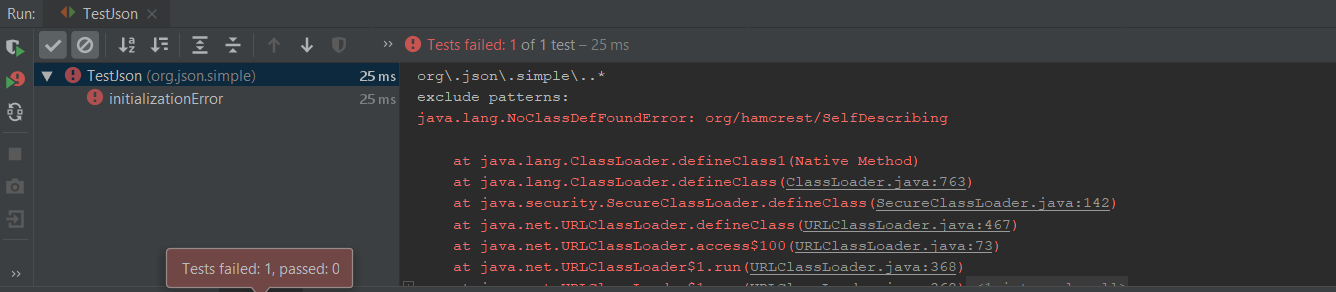
\includegraphics[width=\linewidth]{./img/error.png}
\end{figure}

برای رفع آن باید فایل 
$hamcrest-all-1.3.jar$ 
را به کتاب‌خانه‌های موجود اضافه کنیم.

\begin{figure}[!hbpt]
	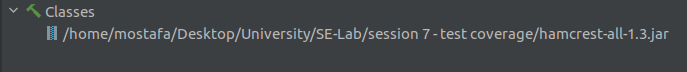
\includegraphics[width=\linewidth]{./img/1.png}
\end{figure}

حال پس از اجرای کد داده‌شده، نتیجه‌ی زیر را می‌گیریم:
\begin{figure}[!hbpt]
	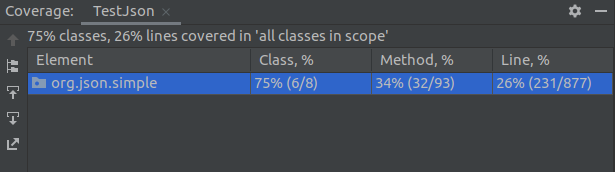
\includegraphics[width=\linewidth]{./img/2.png}
\end{figure}

همان‌طور که در دستور کار آزمایش گفته شده، گزارشی از میزان افزایشی که در اعداد پوشش تست حاصل شده است را به همراه تست‌ها گزارش می‌کنیم:

\begin{figure}[!hbpt]
	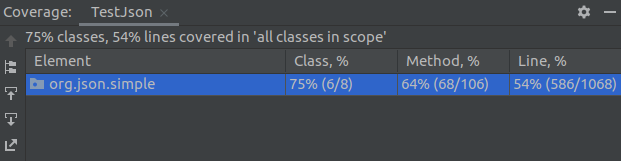
\includegraphics[width=\linewidth]{./img/3.png}
\end{figure}

در هر کدام از تست‌ها یک آبجکت جدید می‌سازیم و در آن منتظر خروجی مد نظرمان را امتحان می‌کنیم. برای مثال در قسمت زیر یک آرایه  $json$ می‌سازیم و توقع داریم که پس از تبدیل آن به رشته خروجی آن برابر با $[]$ باشد.
\begin{Verbatim*}[tabsize=4]
@Test
public void testJSONArray() {
	final JSONArray jsonArray = new JSONArray();
	assertEquals("[]", jsonArray.toJSONString());
}

\end{Verbatim*}

بقیه‌ی مثال‌ها را هم در فایل $TestJson$ آورده‌ایم. (حدود ۱۵ تست)

در نهایت بعد از خروجی گرفتن به صورت فایل $html$ داریم:

\begin{figure}[!hbpt]
	
\includegraphics[width=\linewidth]{./img/4.png}
\end{figure}

	